\documentclass[12pt]{article}

\usepackage[utf8]{inputenc}
\usepackage[russian]{babel}
\usepackage{graphicx}
\usepackage{indentfirst}
\usepackage{booktabs}
\usepackage{amsmath}


\graphicspath{{pic/}}

\begin{document}

\begin{center}
	\LARGE 
	\textbf{Лабораторная работа 2}\\
	Датчики случайных чисел. Построение гистограмм\\
\end{center}

\begin{flushright}
	\large
	Игнашов Иван\\
	Вариант 8\\
\end{flushright}

\newpage

 \section*{1. Цель работы}
Изучение алгоритмов получения на ЭВМ чисел с заданным законом
распределения и построения гистограмм

\subsection*{Порядок работы:}
\begin{enumerate}
	\item Выбрать закон распределения верятностей. В соответствии с вариантом: Эрланговский закон с параметрами $k=3, \lambda=4$
	\item Вывести соотношение, позволяющее из чисел, сформированных базовым
датчиком, получить числа с заданным законом распределения
	\item Написать программу, реализующую датчик случайных чисел с заданным
законом распределения
	\item Написать программу построения гистограммы выборки, сформированной
созданным датчиком с учетом параметров
	\item При помощи программы построения гистограмм заполнить таблицу распределения элементов выборки по квантам гистограммы
	\item На основании таблицы построить гистограмму распределения сформированной выборки
	\item Построить график зависимости оценок математического ожидания и
дисперсии от объема выборки
\end{enumerate}

\newpage
 \section*{2. Формула и график моделируемого закона распределения}%
Плотность вероятности распределения по закону Эрланга:\\
$f(x; k, \lambda) = \frac{\lambda^kx^{k - 1}e^{-\lambda x}}{(k-1)!} $ для $ x,\lambda \geq 0$\\ \\
$f(x; 3, 4) = \frac{64x^{2}e^{-4 x}}{2} = 32x^2e^{-4 x} $ для $ x \geq 0$

 \begin{figure}[!h]
	\centering
	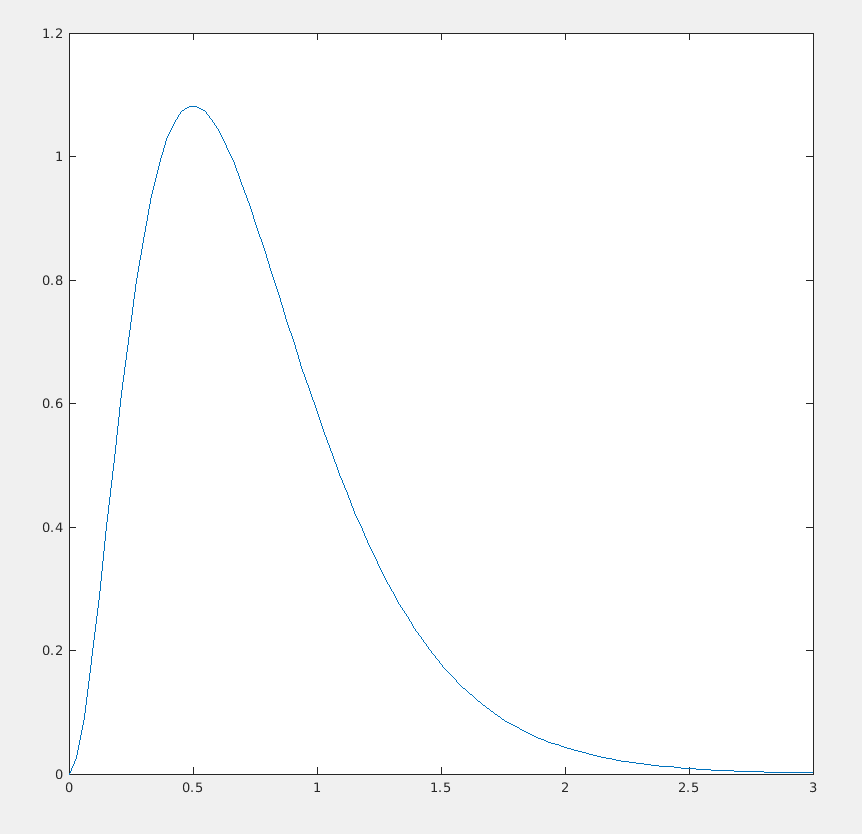
\includegraphics[width=0.5\linewidth]{var8_erlang.png}
	\caption{График закона распределения Эрланга(3,4)}
\end{figure}
 
Для расчета распределения заданной формулы воспользуемся тем, что случайная величина, распределенная по закону Эрланга порядка k и параметром $\lambda$, является суммой k независимых случайных величин, имеющих экспоненциальное распределение с параметром $\lambda$.\\
При этом для экспоненциального закона распределения соотношение выглядит как $a_i = \frac{-1}{\lambda}\ln{R_i}$\\

Таким образом, при k = 3, $\lambda$ = 4 :\\

$a_i^{erl}(k,\lambda) = \sum_{j=1}^3a_j^{exp}(\lambda) = \sum_{j=1}^3\frac{-1}{\lambda}\ln{R_j}$
 
\newpage
 \section*{3. Описание разработанных программ}
 %список использованных переменных, список использованных функций, блок-схема, листинг
 
  \begin{figure}[!h]
	\centering
	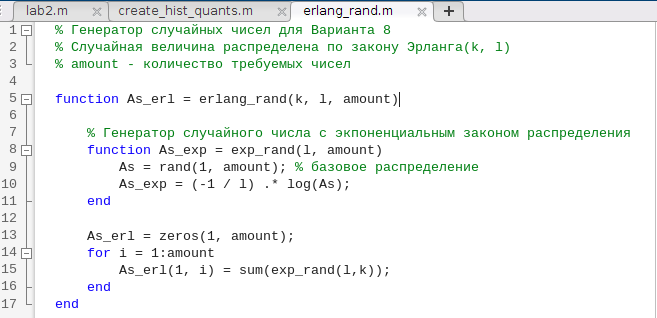
\includegraphics[width=\linewidth]{erlang_rand_code.png}
	\caption{Код генерации случайных значений}
\end{figure}
 
\newpage
 \section*{4. Представление результатов анализа выборки}
 
 \begin{figure}[!h]
	\centering
	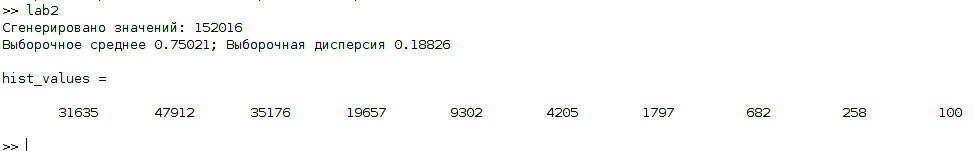
\includegraphics[width=\linewidth]{hist_values_example.png}
	\caption{Пример вывода программы}
\end{figure}

Заполним данными таблицу распределения элементов выборки по квантам гистограммы

\begin{center}
	\begin{tabular}[c]{l|cccccccccc}
  		Номер интервала & 1 & 2 & 3 & 4 & 5 & 6 & 7 & 8 & 9 & 10 \\\hline
  		&&&\\
		Число элементов & 31635 & 41912 & 35176 & 19657 & 9302 & 4205 & 1797 & 682 & 258 & 100\\
	\end{tabular}
\end{center}
 
 \section*{5. Гистограмма сформированной выборки}
 
\begin{figure}[!h]
	\centering
	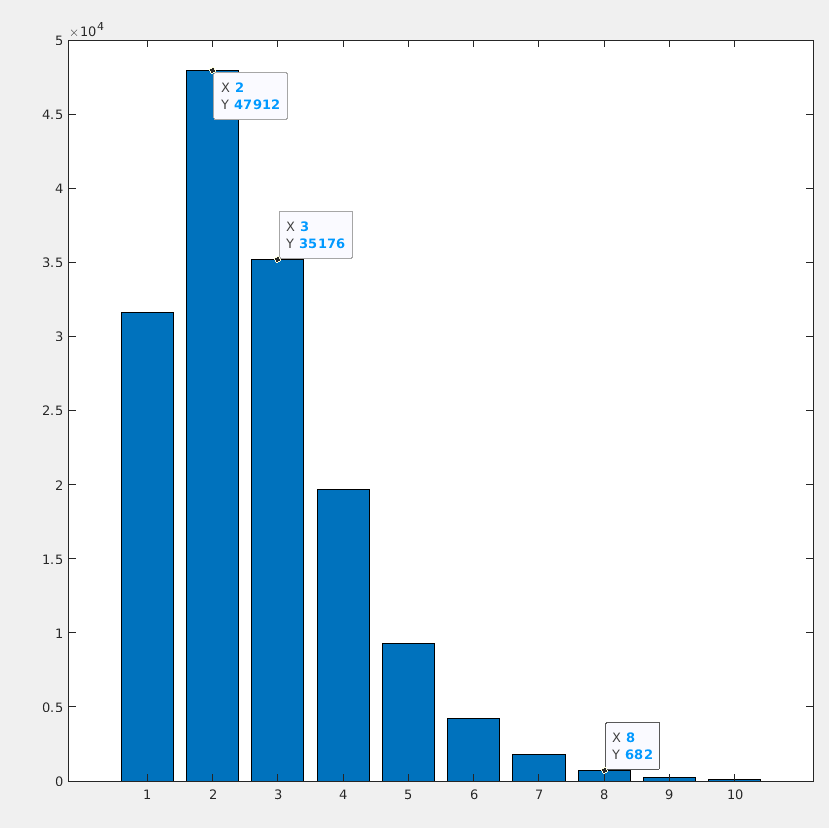
\includegraphics[width=0.5\linewidth]{hist_example.png}
	\caption{Гистограмма для полученной выборки}
\end{figure}

\newpage
 \section*{6. Графики зависимости оценок математического ожидания и дисперсии от объема выборки}
 %На графиках уровнем отметить теоретические значения этиx величин
 
\begin{figure}[!h]
	\centering
	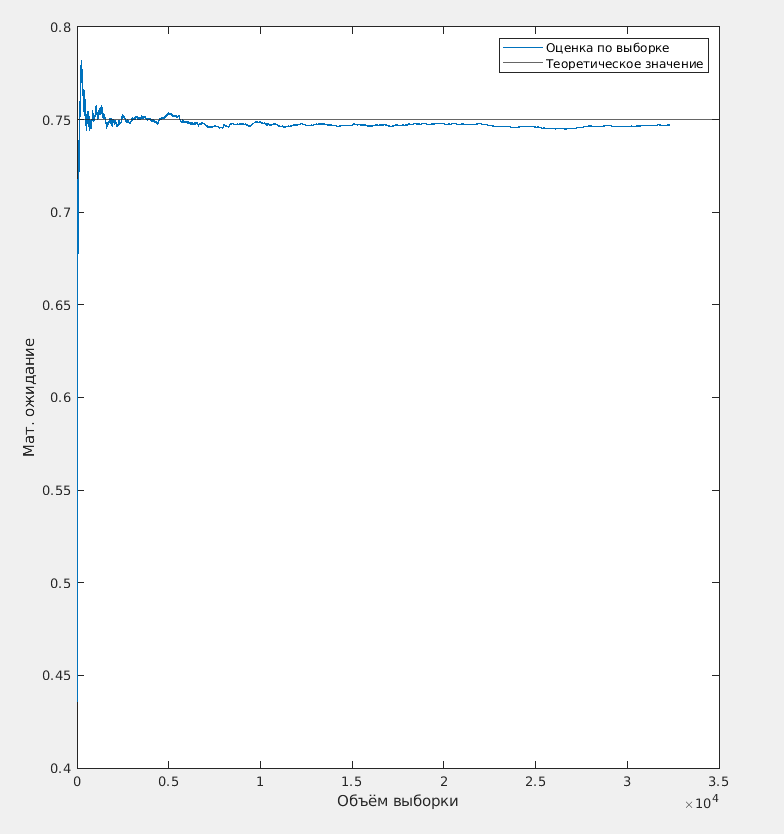
\includegraphics[width=0.5\linewidth]{mean_graph.png}
	\caption{Сравнение значений математического ожидания выборки}
\end{figure}

\begin{figure}[!h]
	\centering
	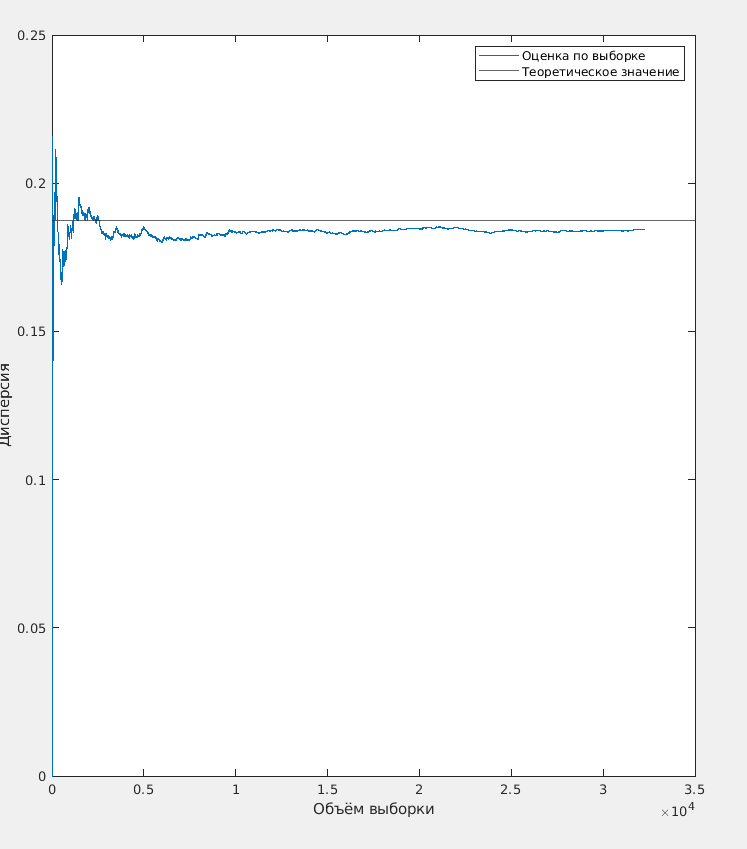
\includegraphics[width=0.5\linewidth]{disp_graph.png}
	\caption{Сравнение значений дисперсии выборки}
\end{figure}

\newpage
 \section*{7. Выводы}
Целью данной лабораторной работы было изучение алгоритмов получения на ЭВМ чисел с заданным законом распределения и построения гистограмм.
В процессе выполнения был реализован способ генерации случайных чисел с эрланговским законом распределения.
Для выборок, полученных данным генератором были построены гистограмма и графики зависимости значений мат. ожидания и дисперсии от объема выборки.

\end{document}